\section{Introduction}

This thesis describes a possible design and a proof-of-concept implementation of a data layer for near real time distributed collaborative applications targeted at operational workloads in small to medium sized businesses with strict auditability requirements.

\paragraph{Context.} The ideas presented in this work are based the author's experience running a \gls{SaaS} business designing and operating an information system in the medical sector for the past five years (see \autoref{fig:rosalind}).


\begin{figure}[!ht]
  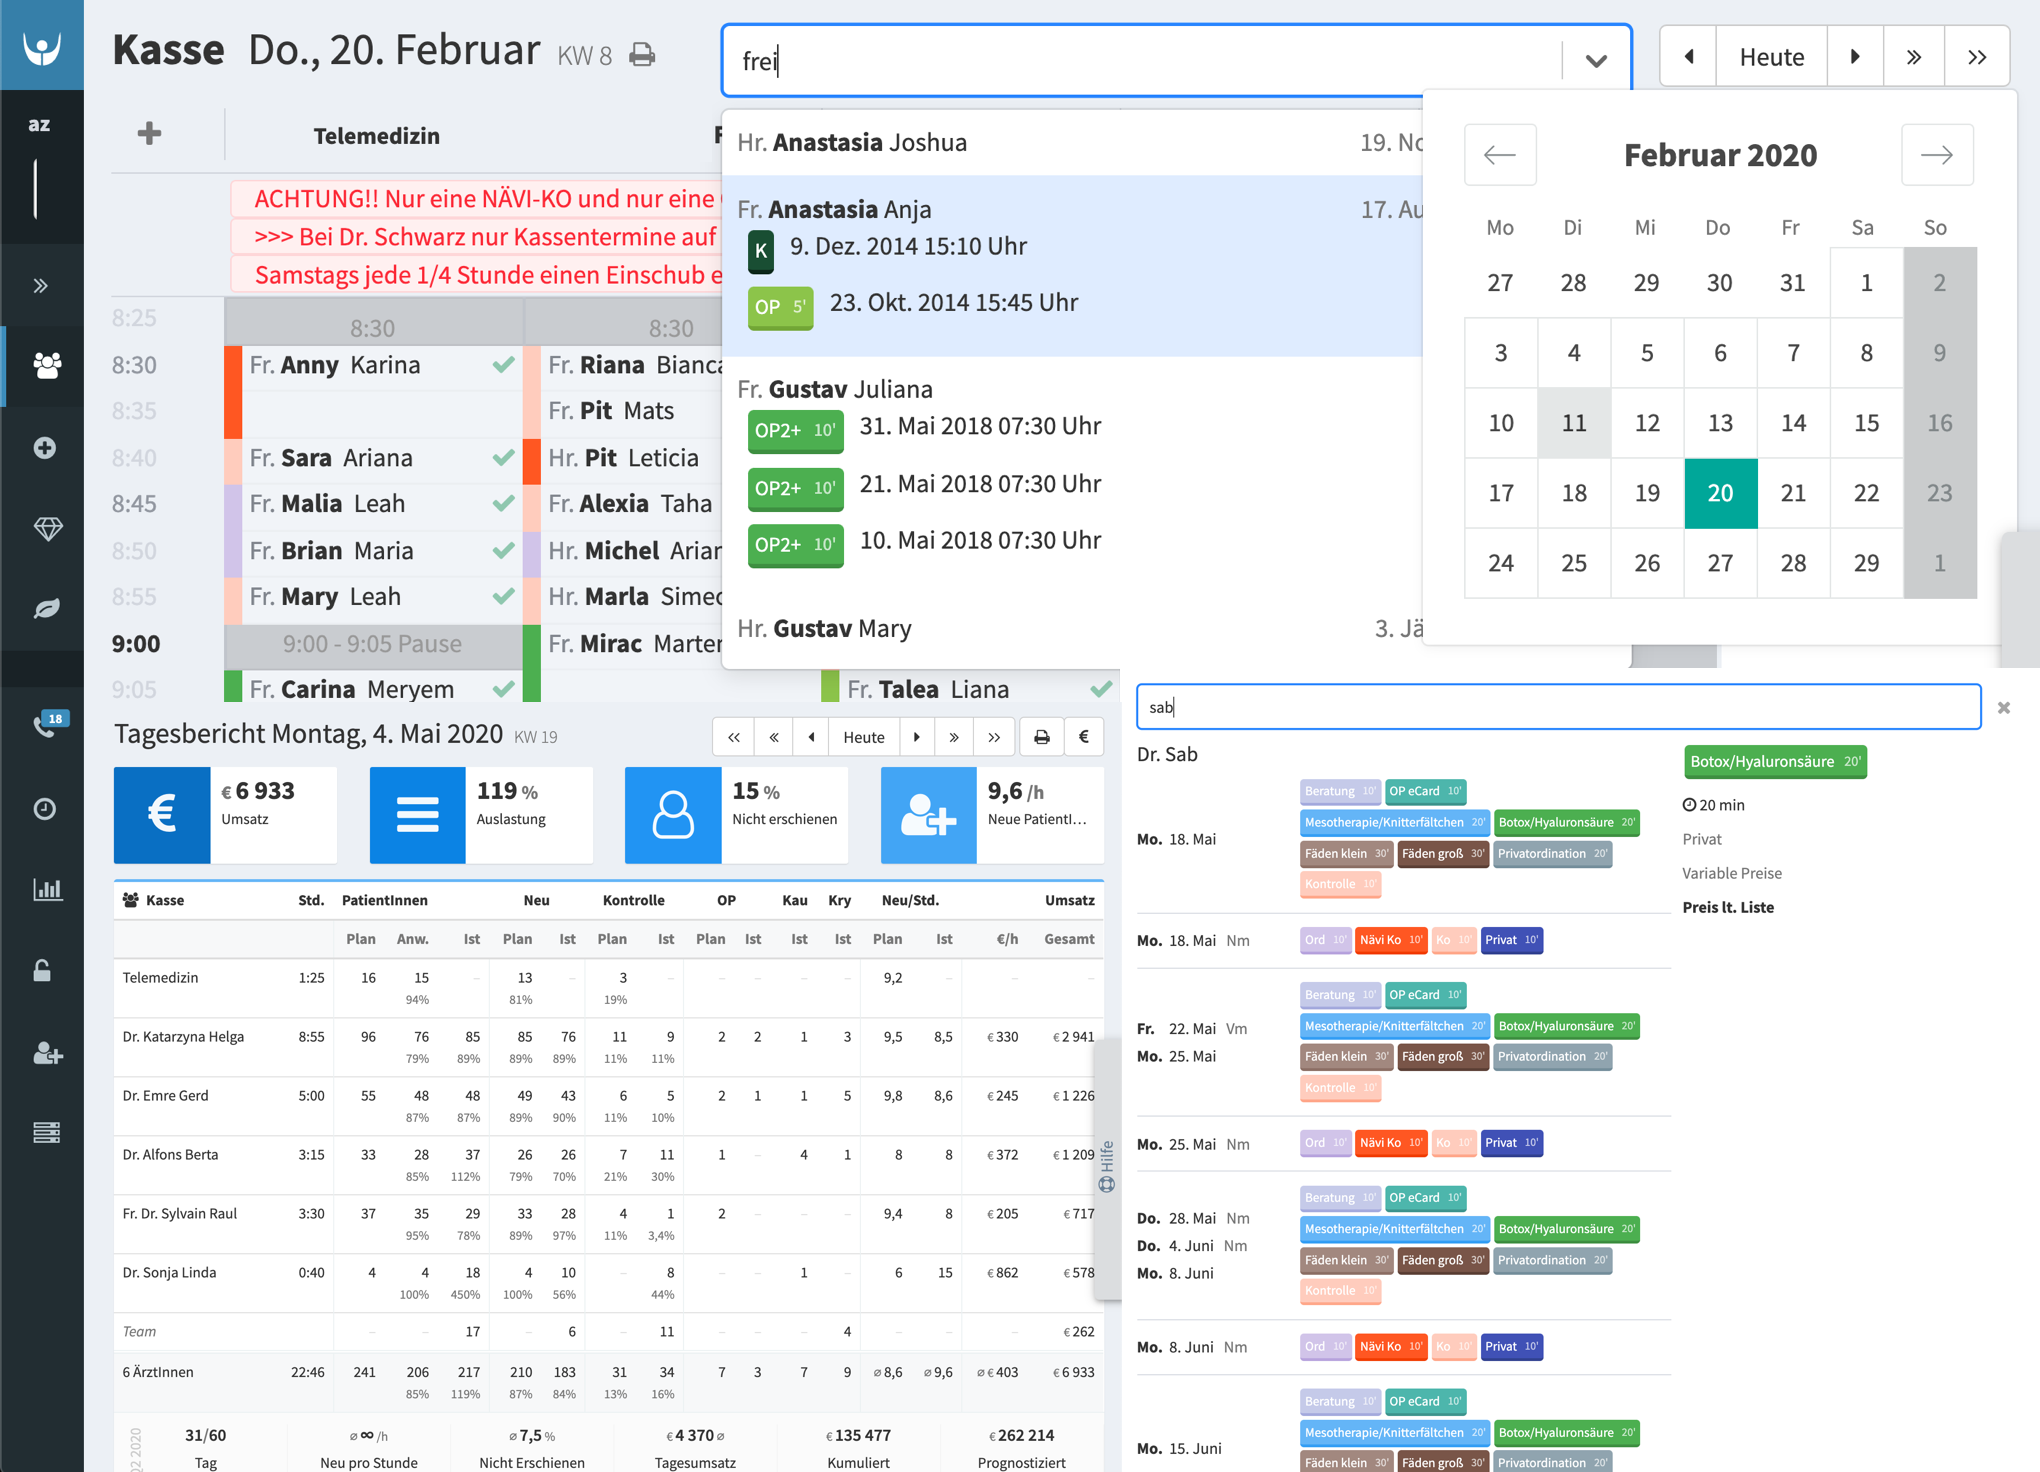
\includegraphics[width=\linewidth]{images/rosalind.png}
  \caption{Composite of the author's medical information system}
  \label{fig:rosalind}
\end{figure}

\paragraph{Outline.} \Cref{sec:related_work} presents related work. \Cref{sec:design} exhibits common problems experienced in data-intensive business applications and shows a different approach towards solving some of them in a functional, immutable, and reactive way. A proof-of-concept implementation is described in \autoref{sec:implementation} and its merits and deficiencies are discussed in \autoref{sec:discussion}.

\cleardoublepage

\subsection{Problem}
Growing customer demands lead to increased incidental complexity \cite{brooks1995mythical} of data-intensive distributed applications \cite{kleppmann2017designing}. \gls{RDBMS}, especially those implementing \gls{SQL} are notable for their focus on performant destructive-by-default write semantics. Modeling inherently complex domains such as healthcare in classic RDBMS leads to an explosion in the number of columns and tables. Their structure has to be known in advance, discouraging an explorative development process. Requirements of real time collaboration, declarative security, auditability of changes, evolution of the schema, and analytics push the limit of established request-response mechanisms.


\subsection{Contribution}
The thesis explains a possible design of a data layer for business applications and describes its prototypal implementation. The core is a simple relational data model based on facts in the form of \gls{EAV} tuples similar to the \gls{6NF} or the \gls{RDF} as seen in Semantic Web literature. Such EAV tuples are kept in an append-only (immutable) log as either assertions or retractions together with two timestamps: \gls{tx} at which the fact was added to the log, and \gls{tv} at which the fact became true in the context of the system \cite{snodgrass1992temporal}.


\paragraph{Goal.}
The goal of this work is to demonstrate the feasibility of an implementation of various desirable features in less than 1000 lines total of readily comprehensible Lisp: Bitemporality, practically immutable audit logging, transaction metadata, server-client reactivity, schemalessness, consistency criteria, versatile automatic indexing, transactions with guarantees of \gls{ACID}, and a simple relational query language based on Datalog.

\paragraph{Method.}
The thesis explains the decisions made while iterating on the design and its implementation and includes a discussion on limitations and advantages.

\paragraph{Results.}
Embracing the EAV+$t_t$+$t_v$ data model together with the expressive programming language ClojureScript \cite{hickey2008clojure} reveals that it is possible to implement a proof-of-concept data layer and query language for business applications with various valuable features not commonly seen in mainstream databases. The implementation is realized using less than 400 lines of code, the majority of which appears to map fairly well to the initial conceptual design.
